\documentclass{article}
\usepackage[utf8]{inputenc}

\title{Software Process - Assignment 2}
\author{
    Jelle van Assema\\
    \and
    Theologos Zacharopoulos\\
    \and
    Guido Loupias\\
    \and 
    Yoan-Alexander Grigorov\\
    \and 
    Jasper Dijt\\
    \and 
    Felix Barten\\
    \and 
    Edward Poot\\ 
    \and 
    Robert Diebels
}
\date{February 2016}

\usepackage{natbib}
\usepackage{graphicx}

\begin{document}

\maketitle

\section{Introduction}
There is a theory which states that if ever anyone discovers exactly what the Universe is for and why it is here, it will instantly disappear and be replaced by something even more bizarre and inexplicable.
There is another theory which states that this has already happened.

\begin{figure}[h!]
\centering
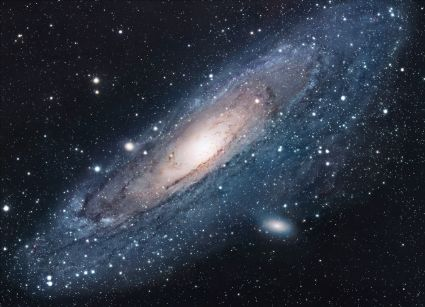
\includegraphics[scale=1.7]{universe.jpg}
\caption{The Universe}
\label{fig:univerise}
\end{figure}

\section{Conclusion}
``I always thought something was fundamentally wrong with the universe'' \citep[All pages]{adams1995hitchhiker}
No comments here?

\bibliographystyle{plain}
\bibliography{references}
\end{document}
